\documentclass[brazil, a4paper]{article}
\usepackage{graphicx}
\usepackage[T1]{fontenc}
\usepackage[utf8]{inputenc}
\usepackage{lmodern}
\usepackage{babel}
\usepackage{url}
\usepackage{listings}
\usepackage{xcolor}
\usepackage{textcomp}

\lstset{language=Python,
	             basicstyle=\footnotesize,
	             numbers=left,
	             numberstyle=\footnotesize,
	             frame=shadowbox,
	             rulesepcolor=\color{blue},
	             showspaces = false, 
		     showstringspaces = false,
	             showtabs = false,
	             }
\begin{document}


\title{Relatório Parcial - Projeto de Aprendizagem Computacional}
\author{Pedro Paulo Vezzá Campos \hfill 7538743\\
		Camila Fernandez Achutti \hfill 6795610}
\date{\today}

\maketitle

%\begin{abstract}
%\end{abstract}


\section{Proposta escolhida}
O grupo optou pela proposta 2, animação de algoritmos de aprendizagem
computacional. O algoritmo a ser implementado e simulado visualmente é o
Perceptron.

\section{Sobre o problema de aprendizagem}
\subsection{PERCEPTRON}
Como explicado no enunciado o Perceptron é um algoritmo de classificação 
supervisionada. Sua principal característica e limitação é que apenas possui 
resultados satisfatórios para a classificação de conjuntos linearmente
separáveis.

Assim, instâncias interessantes para o classificador são conjuntos de dados que
podem ou não ser classificados utilizando uma reta para dividir as categorias
de elementos. O caso clássico de conjunto não linearmente separável é a
função ou-exclusivo (XOR). Dentro dos problemas linearmente separáveis,
é interessante considerar casos em que os pontos de dados estão muito ou
pouco separados para verificar a eficiência do classificador.

Neste trabalho esperamos implementar o perceptron para dimensão arbitrária d $\ge$ 2.

\section{Interface Gráfica}

Foi e será desenvolvida em 2D, ainda que a dimensão d seja maior que 2. Vamos sempre fazer a representação somente de 2 delas. 

A implementação será feita em python e a plotagem será feita usando PyLab e a interface do usuário usando PyGTK.

A entrada pode ser efetuada de 3 maneiras diferentes:
\begin{itemize}
\item marcar os pontos no canvas através de click,
\item ler de um arquivo de entrada, 
\item gerar pontos de forma aleatória.
\end{itemize}

Com o dataset de entrada o algoritmo de aprendizagem entra em jogo e se implementado de forma adequada usa os pontos de amostragem como um conjunto de treinamento para tentar descobrir qual é a linha mais adequada para realizar a classificação. 

A animação mostra como o algoritmo evolui e quais são os ajustes feitos para alcançar o resultado final.

A ferramenta de animação terá as seguintes funcionalidades básicas:
\begin{itemize} 
\item Seleção do modo de entrada: Arquivo, Sorteio, Clique;
\begin{itemize}
\item Arquivo: serão necessários a submissão de dois arquivos diferentes, um de dados de treino e outro de testes. Ambos são csv's de 3 colunas. 
\item Sorteio: dados aleátorios são gerados, somente com o controle de serem gerados dois conjuntos linearmente separáveis.

\end{itemize}
\item Botão de 'TREINAR' para que o algoritmo comece a rodar, ao final do algorimo ele pode ser novamente apertado para que o treinamento seja refeito;
\item Botão 'TESTAR' para que o conjunto de teste seja plotado e o resultado possa ser validado pelo usuário;
\item Possibilidade de  ajustar o valor de $\eta$ (taxa de aprendizagem) para controlar a rapidez com que o perceptron aprende;
\item Definição do número máximo de iterações, onde uma iteração representa a atualização do vetor de pesos a cada ponto que é analisado, sendo assim, se a reta inicial arbitrária for correta, encontramos a solução em 0 iterações do algoritmo.
\end{itemize}

A taxa de aprendizagem é a que dimensiona o vetor de treinamento antes de ser adicionado ao vetor de peso durante as atualizações. Experimente valores diferentes, se quiser, valores maiores afetará a taxa de convergência, mas não a própria convergência. 

O número de iterações é colocado de modo que o algoritmo não será executado para sempre se os vetores de entrada não são separáveis. 

Normalmente, um valor maior de $\eta$ fará com que ele encontre uma solução mais rapidamente, mas pode causar a perda de soluções de casos difíceis. E a definição do número máximo de iteração garante que o algoritmo vai ter fim, ainda que não encontre um solução de erro global nulo.

A sequência esperada do usuário e da animação é a seguinte:
\begin{enumerate}
\item seleção do modo de entrada
\item plotagem do conjunto de treinamento 
\item click do usuário no botão 'TREINAR'
\item plotagem das retas que o algoritmo encontrou durante a execução 
\item click no botão 'TESTAR' para que o conjunto de teste seja plotado e o algoritmo possa ser avaliado pelo usuário.
\end{enumerate}
O botão de 'REINICIAR' pode ser usado para que o algoritmo refaça o treinamento com os mesmos dados, mas com a possibilidade de trocar os parâmetros.

\section{Cronograma Proposto}
Na tabela a seguir estão listadas as tarefas a serem cumpridas para o projeto
de MAC0460 de 2013:

\begin{table}[h]
    \begin{tabular}{|p{5cm}|c|c|c|c|}
    \hline
    Atividade                                                       & setembro & outubro & novembro & dezembro \\ \hline
    Implementar o Perceptron                                        & X        & ~       & ~        & ~        \\
    Buscar na Internet e testar entradas interessantes como exemplo & X        & X       & ~        & ~        \\
    Implementar a interface gráfica                                 & X        & X       & X        & ~        \\
    Escrever o relatório parcial                                    & ~        & X       & ~        & ~        \\ 
    Escrever o relatório final                                      & ~        & ~       & X        & X        \\ \hline
    \end{tabular}
    \caption{Cronograma das tarefas a serem realizadas no semestre}
\end{table}

O cronograma proposto foi cumprido e não sofreu qualquer alteração.

\section{O que já foi feito}

\begin{itemize}
\item {\bf Estudo e implementação do algoritmo perceptron em Python}

Realizamos um estudo detalhado do funcionamento do algoritmo  e realizamos a seguinte implementação simplificada em Python:

\lstinputlisting{perceptron.py}

Nesse algoritmo limitamos o número máximo de iterações em 100 e $\eta$ para efeito de teste.

\item {\bf Busca de exemplos interessantes para teste da animação}

\begin{itemize}
\item XOR
	O exemplo aqui é a função XOR. Nele não é possível traçar uma única reta (função linear) tal que divida o plano de maneira que as saídas com valor 0 ficam situadas de um lado da reta e as com valor 1 do outro. Entretanto, este problema pode ser solucionado com a criação de uma camada intermediária na rede e graficamente com uma estrutura em três (ou mais) dimensões.
	\newpage
		\begin{table}[h]
			\centering
			\begin{tabular}{|c|c|c|}
			\hline
			x1 & x2 & u \\ \hline
			0 & 0 & 0 \\
			0 & 1 & 1 \\
			1 & 0 & 1 \\
			1 & 1 & 0 \\ \hline
			\end{tabular}
			\caption{Conjunto de treinamento do exemplo XOR}
		\end{table}
		
	\item Violeta para exportação
	
	Neste exemplo temos que classificar violetas para serem importadas e as que vão ficar no mercado. 
	
	As violetas são classificadas de acordo com uma escala de intensidade de cor que vai de 1 a 8 e outra escala de textura que vai de 1 a 5.
	
	Definimos que a classe 1 é a de exportacão e a classe 2 é a para mercado interno e temos o seguinte conjunto de teste:
	\begin{table}[h]
			\centering
			\begin{tabular}{|c|c|c|}
			\hline
			cor & textura & classe \\ \hline
			4 &5 & 1 \\
			5 & 4 & 1 \\
			6 & 3 & 1 \\
			7 & 1 & 1 \\
			8 & 2 & 1 \\
			1 & 3 & 2 \\
			1 & 5 & 2 \\
			2 & 2 & 2 \\
			3 & 4 & 2 \\
			4 & 2 & 2 \\ \hline
			\end{tabular}
			\caption{Conjunto de treinamento do exemplo das violetas}
		\end{table}

	\begin{table} [h]
			\centering
			\begin{tabular}{|c|c|c|}
			\hline
			cor & textura & classe \\ \hline
			5 & 1 & 1 \\
			5 & 3 & 2 \\
			6 & 2 & 1 \\ \hline
			\end{tabular}
			\caption{Conjunto de teste do exemplo das violetas}
		\end{table}
\end{itemize}

\item Implementar interface gráfica

A interface gráfica já desenvolvida se restringe a exibição dos pontos de treinamento e teste e das linhas obtidas durante o treinamento.

Assim que o programa rodar ele abre uma janela como ilustrada abaixo e a interface com o usuário já está implementada para suportar sequências de cliques errados.

\newpage

\begin{figure}[!htb]
\centering
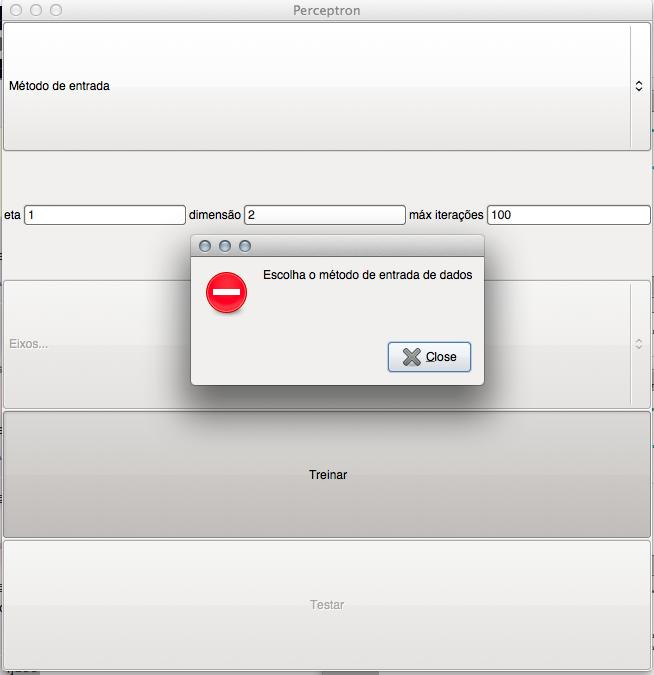
\includegraphics[scale=0.25]{erro.png}
\caption{Interface com o usuário.}
\end{figure}

Se escolhermos sortear os dados o nosso aplicativo se comporta da seguinte maneira representada pela sequência de fotos abaixo:

\begin{figure}[!htb]
\centering
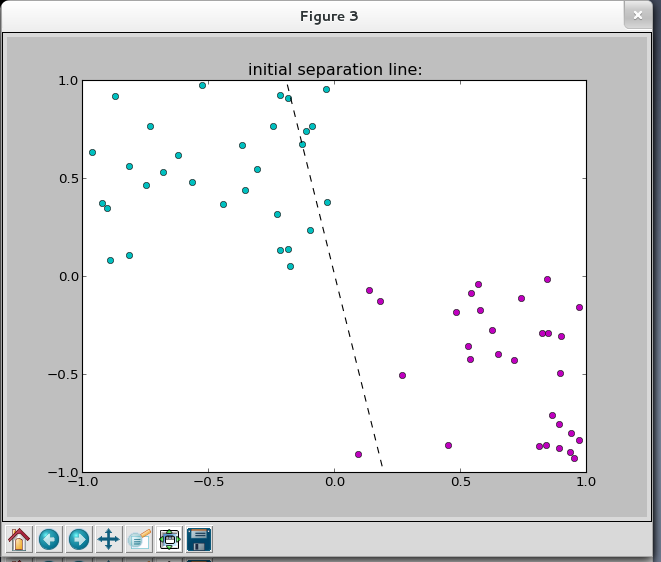
\includegraphics[scale=0.25]{ex1-1.png}
\caption{Situação inicial do exemplo 1, onde uma reta arbitrária foi sorteada.}
\end{figure}

\newpage

\begin{figure}[!htb]
\centering
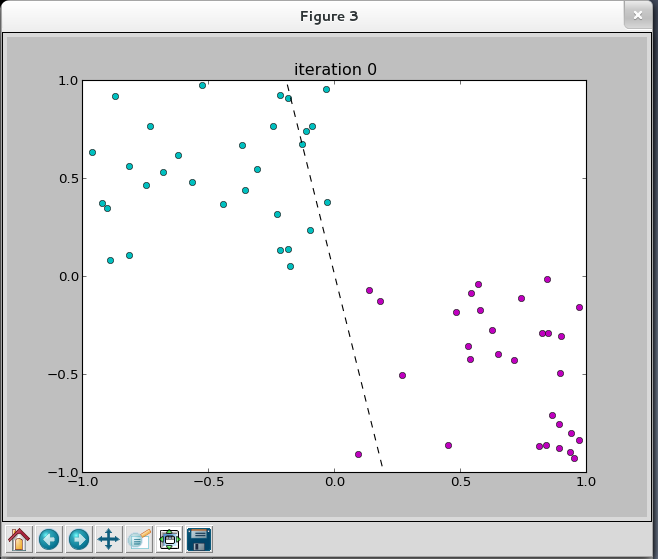
\includegraphics[scale=0.25]{ex1-2.png}
\caption{Começa a execução do algoritmo para o exemplo 1.}
\end{figure}

\begin{figure}[!htb]
\centering
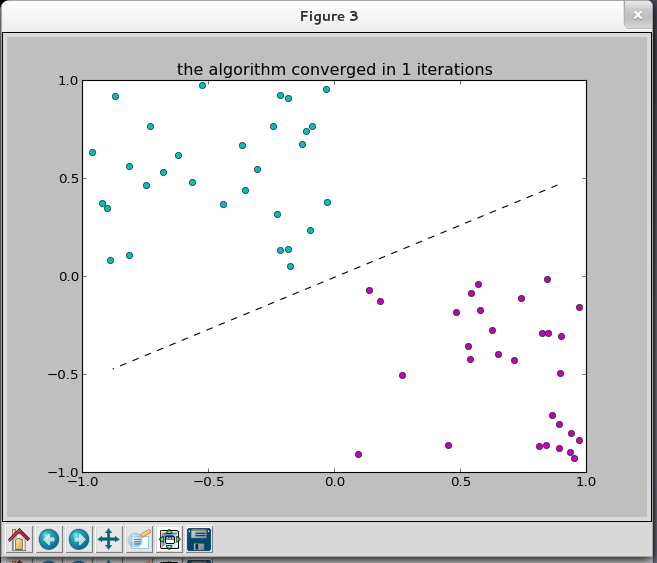
\includegraphics[scale=0.25]{ex1-3.png}
\caption{Fim do algoritmo, reta classificadora foi encontrada no exemplo 1.}
\end{figure}

Agora queremos mostrar como é feito o teste, que é quando o usuário clica no botão TESTAR. Lembrando que só será valido se ele já tiver realizado o treino.

\newpage

\begin{figure}[!htb]
\centering
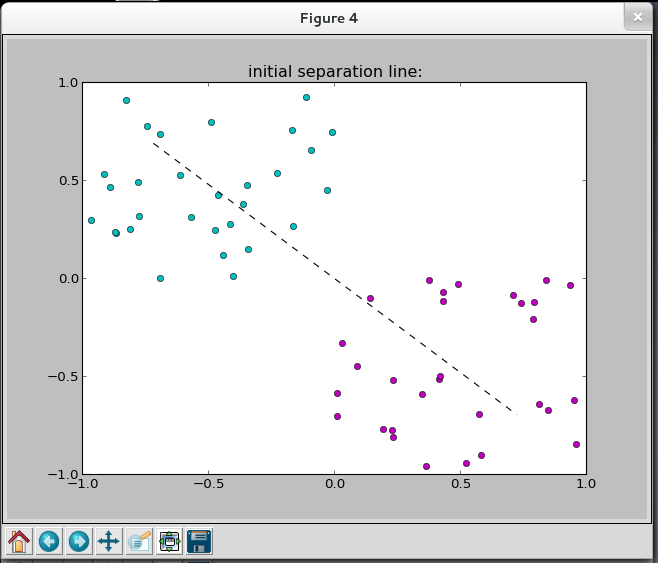
\includegraphics[scale=0.25]{ex2-1.png}
\caption{Situação inicial do exemplo 2, onde uma reta arbitrária foi sorteada.}
\end{figure}

\begin{figure}[!htb]
\centering
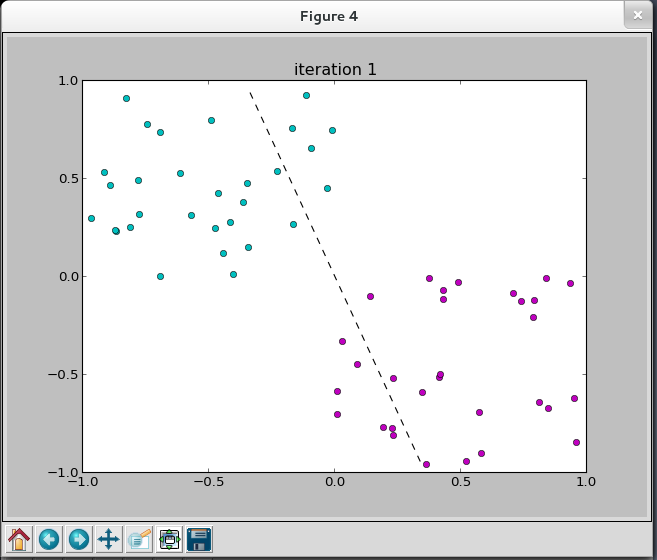
\includegraphics[scale=0.25]{ex2-2.png}
\caption{Começa a execução do algoritmo para o exemplo 2.}
\end{figure}

\newpage

\begin{figure}[!htb]
\centering
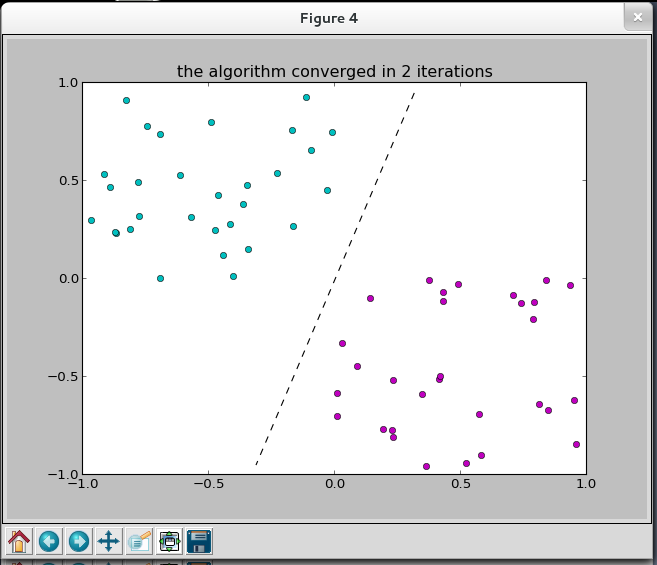
\includegraphics[scale=0.25]{ex2-3.png}
\caption{Fim do algoritmo, reta classificadora foi encontrada para o exemplo 2.}
\end{figure}

Agora se o usuário apertar o botão TESTAR os dados de treino serão retirados do gráfico e os dados de teste serão colocados conforme ilustrado nas imagens abaixo:

\begin{figure}[!htb]
\centering
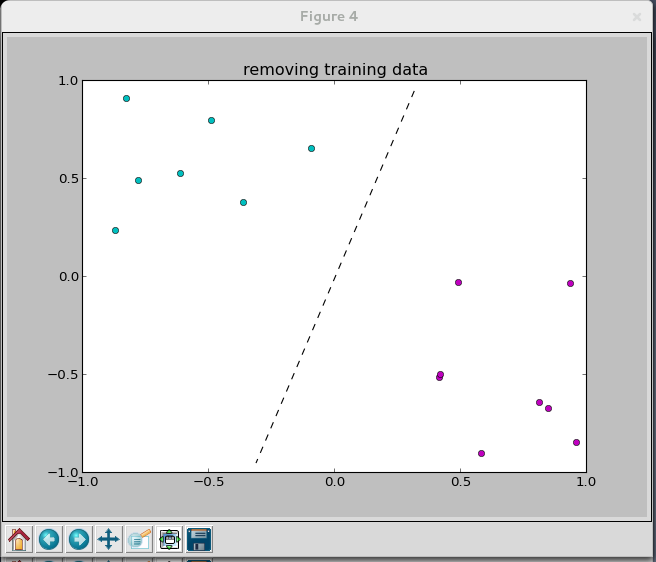
\includegraphics[scale=0.25]{ex2-t1.png}
\caption{Remoção dos dados de treino.}
\end{figure}

\newpage

\begin{figure}[!htb]
\centering
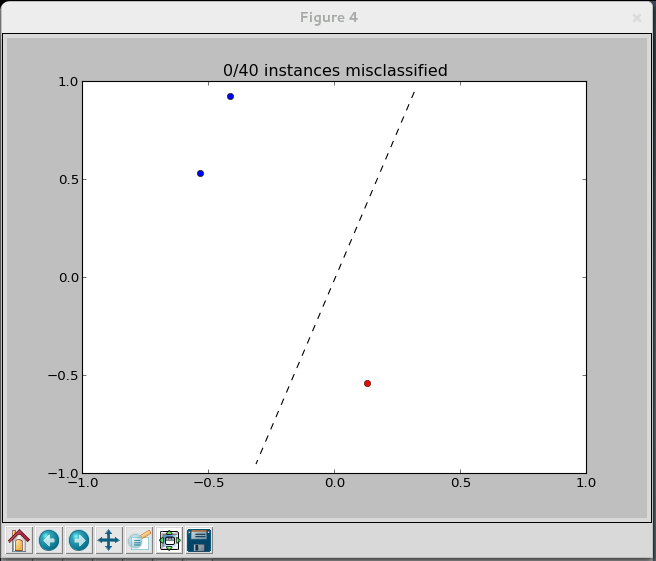
\includegraphics[scale=0.25]{ex2-t2.png}
\caption{Exibição dos dados de teste.}
\end{figure}

\begin{figure}[!htb]
\centering
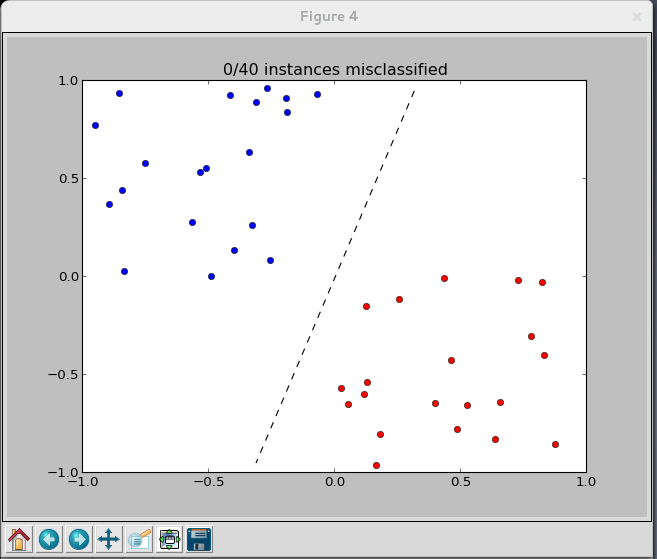
\includegraphics[scale=0.25]{ex2-t3.png}
\caption{Fim do teste para o exemplo 2.}
\end{figure}

Neste caso apresentado acima temos um treinamento bem sucedido. Agora vamos ilustrar uma caso de treinamento mal-sucedido. Para isso alteramos o eta para um valor baixo para que a taxa de aprendizado fosse bem baixa e limitamos o número de iterações para 1. O resultado obtido está ilustrado abaixo: 

\newpage

\begin{figure}[!htb]
\centering
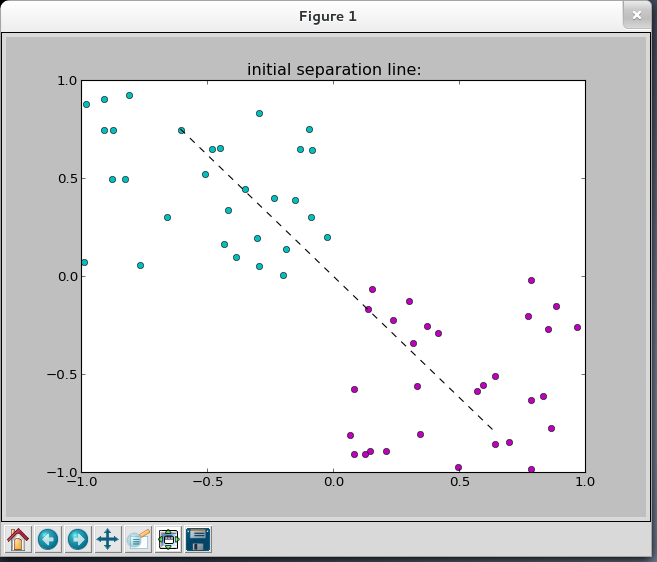
\includegraphics[scale=0.25]{ex3-1.png}
\caption{Exibição dos dados de teste.}
\end{figure}

\begin{figure}[!htb]
\centering
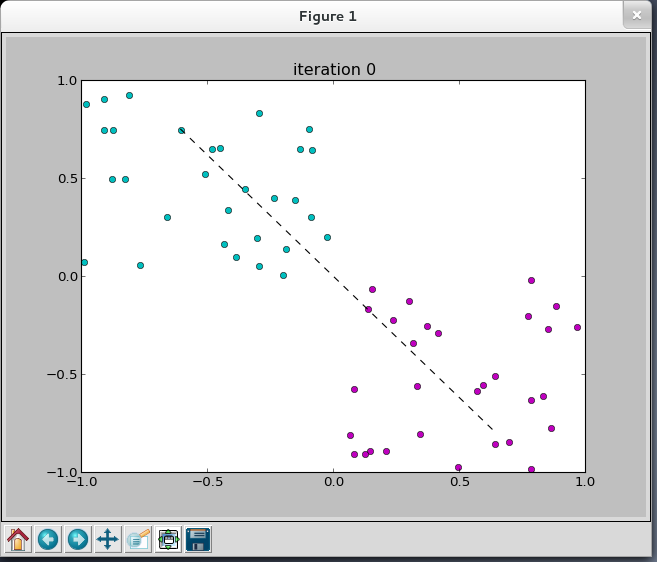
\includegraphics[scale=0.25]{ex3-2.png}
\caption{Fim do teste para o exemplo 2.}
\end{figure}

\newpage

\begin{figure}[!htb]
\centering
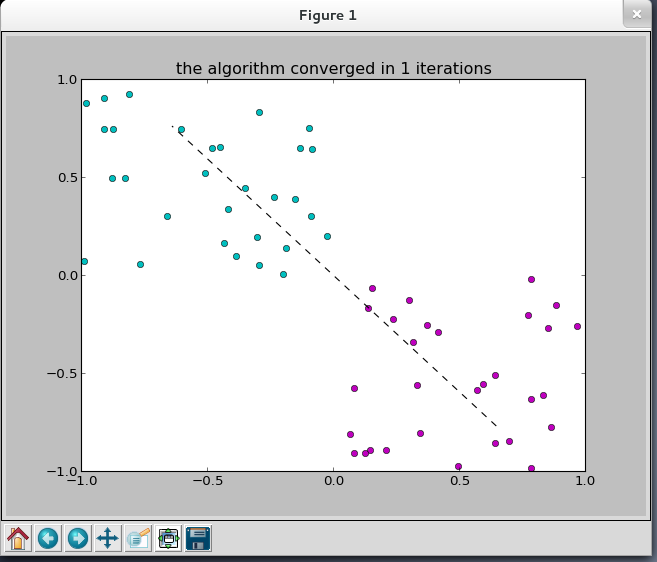
\includegraphics[scale=0.25]{ex3-3.png}
\caption{Exibição dos dados de teste.}
\end{figure}

\begin{figure}[!htb]
\centering
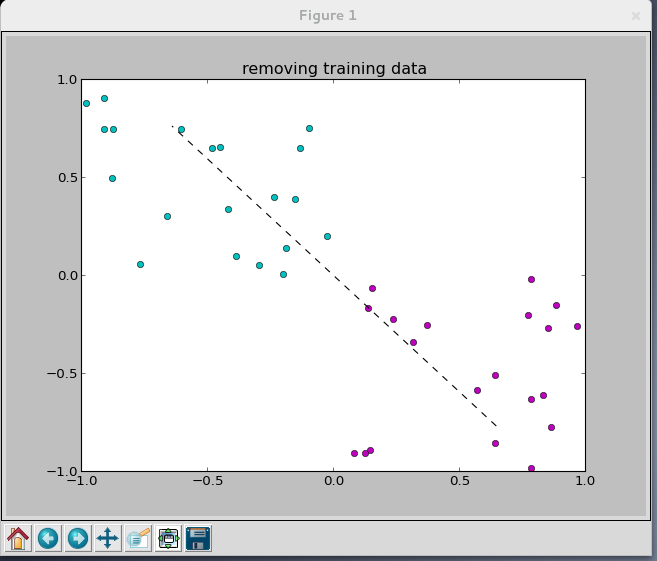
\includegraphics[scale=0.25]{ex3-4.png}
\caption{Fim do teste para o exemplo 2.}
\end{figure}

\newpage
\begin{figure}[!htb]
\centering
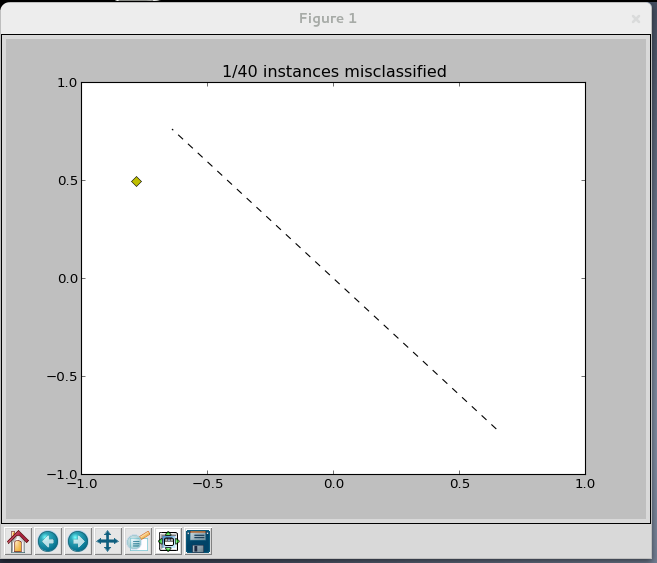
\includegraphics[scale=0.25]{ex3-t1.png}
\caption{Exibição dos dados de teste.}
\end{figure}

\begin{figure}[!htb]
\centering
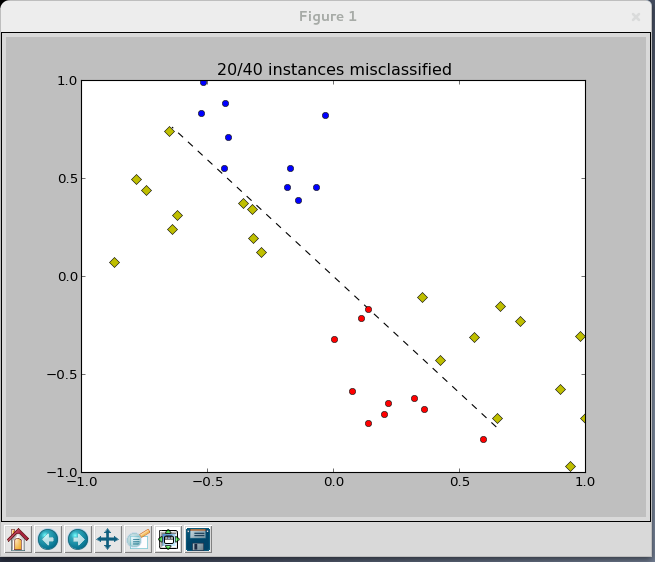
\includegraphics[scale=0.25]{ex3-t2.png}
\caption{Fim do teste para o exemplo 3.}
\end{figure}


Aqui esclarecemos que o diamante amarelo representa os dados de teste mal classificados de ambas as amostras.

É possível também realizar a entrada de dados por arquivos externos. Devem ser produzidos e carregados dois arquivos separados um de treinamento e outro de teste, ambos no formato CSV com o seguinte padrão: \texttt{x1, x2, classe}, onde a classe é 1 ou -1.
\end{itemize} 

\section{O que falta ser feito}

\begin{itemize}
\item Estudo e implementação do algoritmo perceptron em Python

Falta a implementação do algoritmo para mais de duas dimensões.

\item Implementar interface gráfica

Falta a implementação da interface com o usuário que permitirá a seleção do método de entrada por clique.
 
\item Escrever Relatório Final

A redação do relatório final será iniciada em novembro conforme consta no cronograma. 

\end{itemize}  

\section{Bibliografia}
\begin{itemize}
\item http://computing.dcu.ie/~humphrys/Notes/Neural/single.neural.html
\item http://eecs.wsu.edu/~cook/ai/lectures/applets/perceptron/
\item http://matplotlib.org/
\item http://www.pygtk.org/
\end{itemize}
\end{document}

